%%%%%%%%%%%%%%%%%%%%%%%%%%%%%%%%%%%%%%%%%%%%%%%%%%%%%%%%%%%%%%%%%%%%%%%%%%%%%%%%
%%%%%%%%%%%%%%%%%%   Vorlage für eine Abschlussarbeit   %%%%%%%%%%%%%%%%%%%%%%%%
%%%%%%%%%%%%%%%%%%%%%%%%%%%%%%%%%%%%%%%%%%%%%%%%%%%%%%%%%%%%%%%%%%%%%%%%%%%%%%%%

% Erstellt von Maximilian Nöthe, <maximilian.noethe@tu-dortmund.de>
% ausgelegt für lualatex und Biblatex mit biber

% Kompilieren mit 
% latexmk --lualatex --output-directory=build thesis.tex
% oder einfach mit:
% make

\documentclass[
  tucolor,       % remove for less green,
  BCOR=12mm,     % 12mm binding corrections, adjust to fit your binding
  parskip=half,  % new paragraphs start with half line vertical space
  open=any,      % chapters start on both odd and even pages
  cleardoublepage=plain,  % no header/footer on blank pages
]{tudothesis}


% Warning, if another latex run is needed
\usepackage[aux]{rerunfilecheck}

% just list chapters and sections in the toc, not subsections or smaller
\setcounter{tocdepth}{2}

%------------------------------------------------------------------------------
%------------------------------ Fonts, Unicode, Language ----------------------
%------------------------------------------------------------------------------
\usepackage{fontspec}
\defaultfontfeatures{Ligatures=TeX}  % -- becomes en-dash etc.

% language
\usepackage{polyglossia}
\setdefaultlanguage{english}

% for english abstract and english titles in the toc
\setotherlanguages{english}

% intelligent quotation marks, language and nesting sensitive
\usepackage[autostyle]{csquotes}

% microtypographical features, makes the text look nicer on the small scale
\usepackage{microtype}

%------------------------------------------------------------------------------
%------------------------ Math Packages and settings --------------------------
%------------------------------------------------------------------------------

\usepackage{amsmath}
\usepackage{amssymb}
\usepackage{mathtools}

% Enable Unicode-Math and follow the ISO-Standards for typesetting math
\usepackage[
  math-style=ISO,
  bold-style=ISO,
  sans-style=italic,
  nabla=upright,
  partial=upright,
]{unicode-math}
\setmathfont{Latin Modern Math}

% nice, small fracs for the text with \sfrac{}{}
\usepackage{xfrac}  


%------------------------------------------------------------------------------
%---------------------------- Numbers and Units -------------------------------
%------------------------------------------------------------------------------

\usepackage[
  separate-uncertainty=true,
  per-mode=symbol-or-fraction,
]{siunitx}
\sisetup{math-micro=\text{µ},text-micro=µ}

%------------------------------------------------------------------------------
%-------------------------------- tables  -------------------------------------
%------------------------------------------------------------------------------

\usepackage{booktabs}       % \toprule, \midrule, \bottomrule, etc

%------------------------------------------------------------------------------
%-------------------------------- graphics -------------------------------------
%------------------------------------------------------------------------------

\usepackage{graphicx}
% currently broken
% \usepackage{grffile}

% allow figures to be placed in the running text by default:
\usepackage{scrhack}
\usepackage{float}
\floatplacement{figure}{htbp}
\floatplacement{table}{htbp}

% keep figures and tables in the section
\usepackage[section, below]{placeins}

\usepackage{tikz}

%------------------------------------------------------------------------------
%---------------------- customize list environments ---------------------------
%------------------------------------------------------------------------------

\usepackage{enumitem}

%------------------------------------------------------------------------------
%------------------------------ Bibliographie ---------------------------------
%------------------------------------------------------------------------------

\usepackage[
  backend=biber,   % use modern biber backend
  autolang=hyphen, % load hyphenation rules for if language of bibentry is not
                   % german, has to be loaded with \setotherlanguages
                   % in the references.bib use langid={en} for english sources
]{biblatex}
\addbibresource{references.bib}  % the bib file to use
\DefineBibliographyStrings{german}{andothers = {{et\,al\adddot}}}  % replace u.a. with et al.


% Last packages, do not change order or insert new packages after these ones
\usepackage[pdfusetitle, unicode, linkbordercolor=tugreen]{hyperref}
\usepackage{bookmark}
\usepackage[shortcuts]{extdash}

%------------------------------------------------------------------------------
%-------------------------    Angaben zur Arbeit   ----------------------------
%------------------------------------------------------------------------------

\author{Lukas Beiske}
\title{High-level Event Reconstruction for the LST-1 Prototype of the Cherenkov Telescope Array}
\date{2020}
\birthplace{Hamm}
\chair{Lehrstuhl für Experimentelle Physik V}
\division{Fakultät Physik}
\thesisclass{Bachelor of Science}
\submissiondate{18. August 2020}
\firstcorrector{Prof.~Dr.~Dr.~Wolfgang Rhode}
\secondcorrector{Prof.~Dr.~Kevin Kröninger}

% tu logo on top of the titlepage
\titlehead{
\includegraphics[height=1.5cm]{images/tu-logo.pdf}}

\begin{document}
\frontmatter
\maketitle

% Gutachterseite
\makecorrectorpage

% hier beginnt der Vorspann, nummeriert in römischen Zahlen
\thispagestyle{plain}

\section*{Kurzfassung}
Hier steht eine Kurzfassung der Arbeit in deutscher Sprache inklusive der Zusammenfassung der
Ergebnisse.
Zusammen mit der englischen Zusammenfassung muss sie auf diese Seite passen.

\section*{Abstract}
\begin{english}
The abstract is a short summary of the thesis in English, together with the German summary it has to fit on this page.
\end{english}

\tableofcontents

\mainmatter
% Hier beginnt der Inhalt mit Seite 1 in arabischen Ziffern
\chapter{Gamma-Ray Astronomy}
In astronomy observations can be conducted using many different particles emitted by cosmic sources. 
These particles not only include photons from the whole energy spectrum from the lowest radio up until the highest energy gamma ray domain,
but also neutrions and particles carrying electrical charge like protons or ions (see \autoref{fig:mma}). 
Recently it even became possible to detect gravitational waves emitted by vergy highly energetic events like the merging of two black holes \cite{PhysRevLett.116.061102}.
\begin{figure}
    \centering
    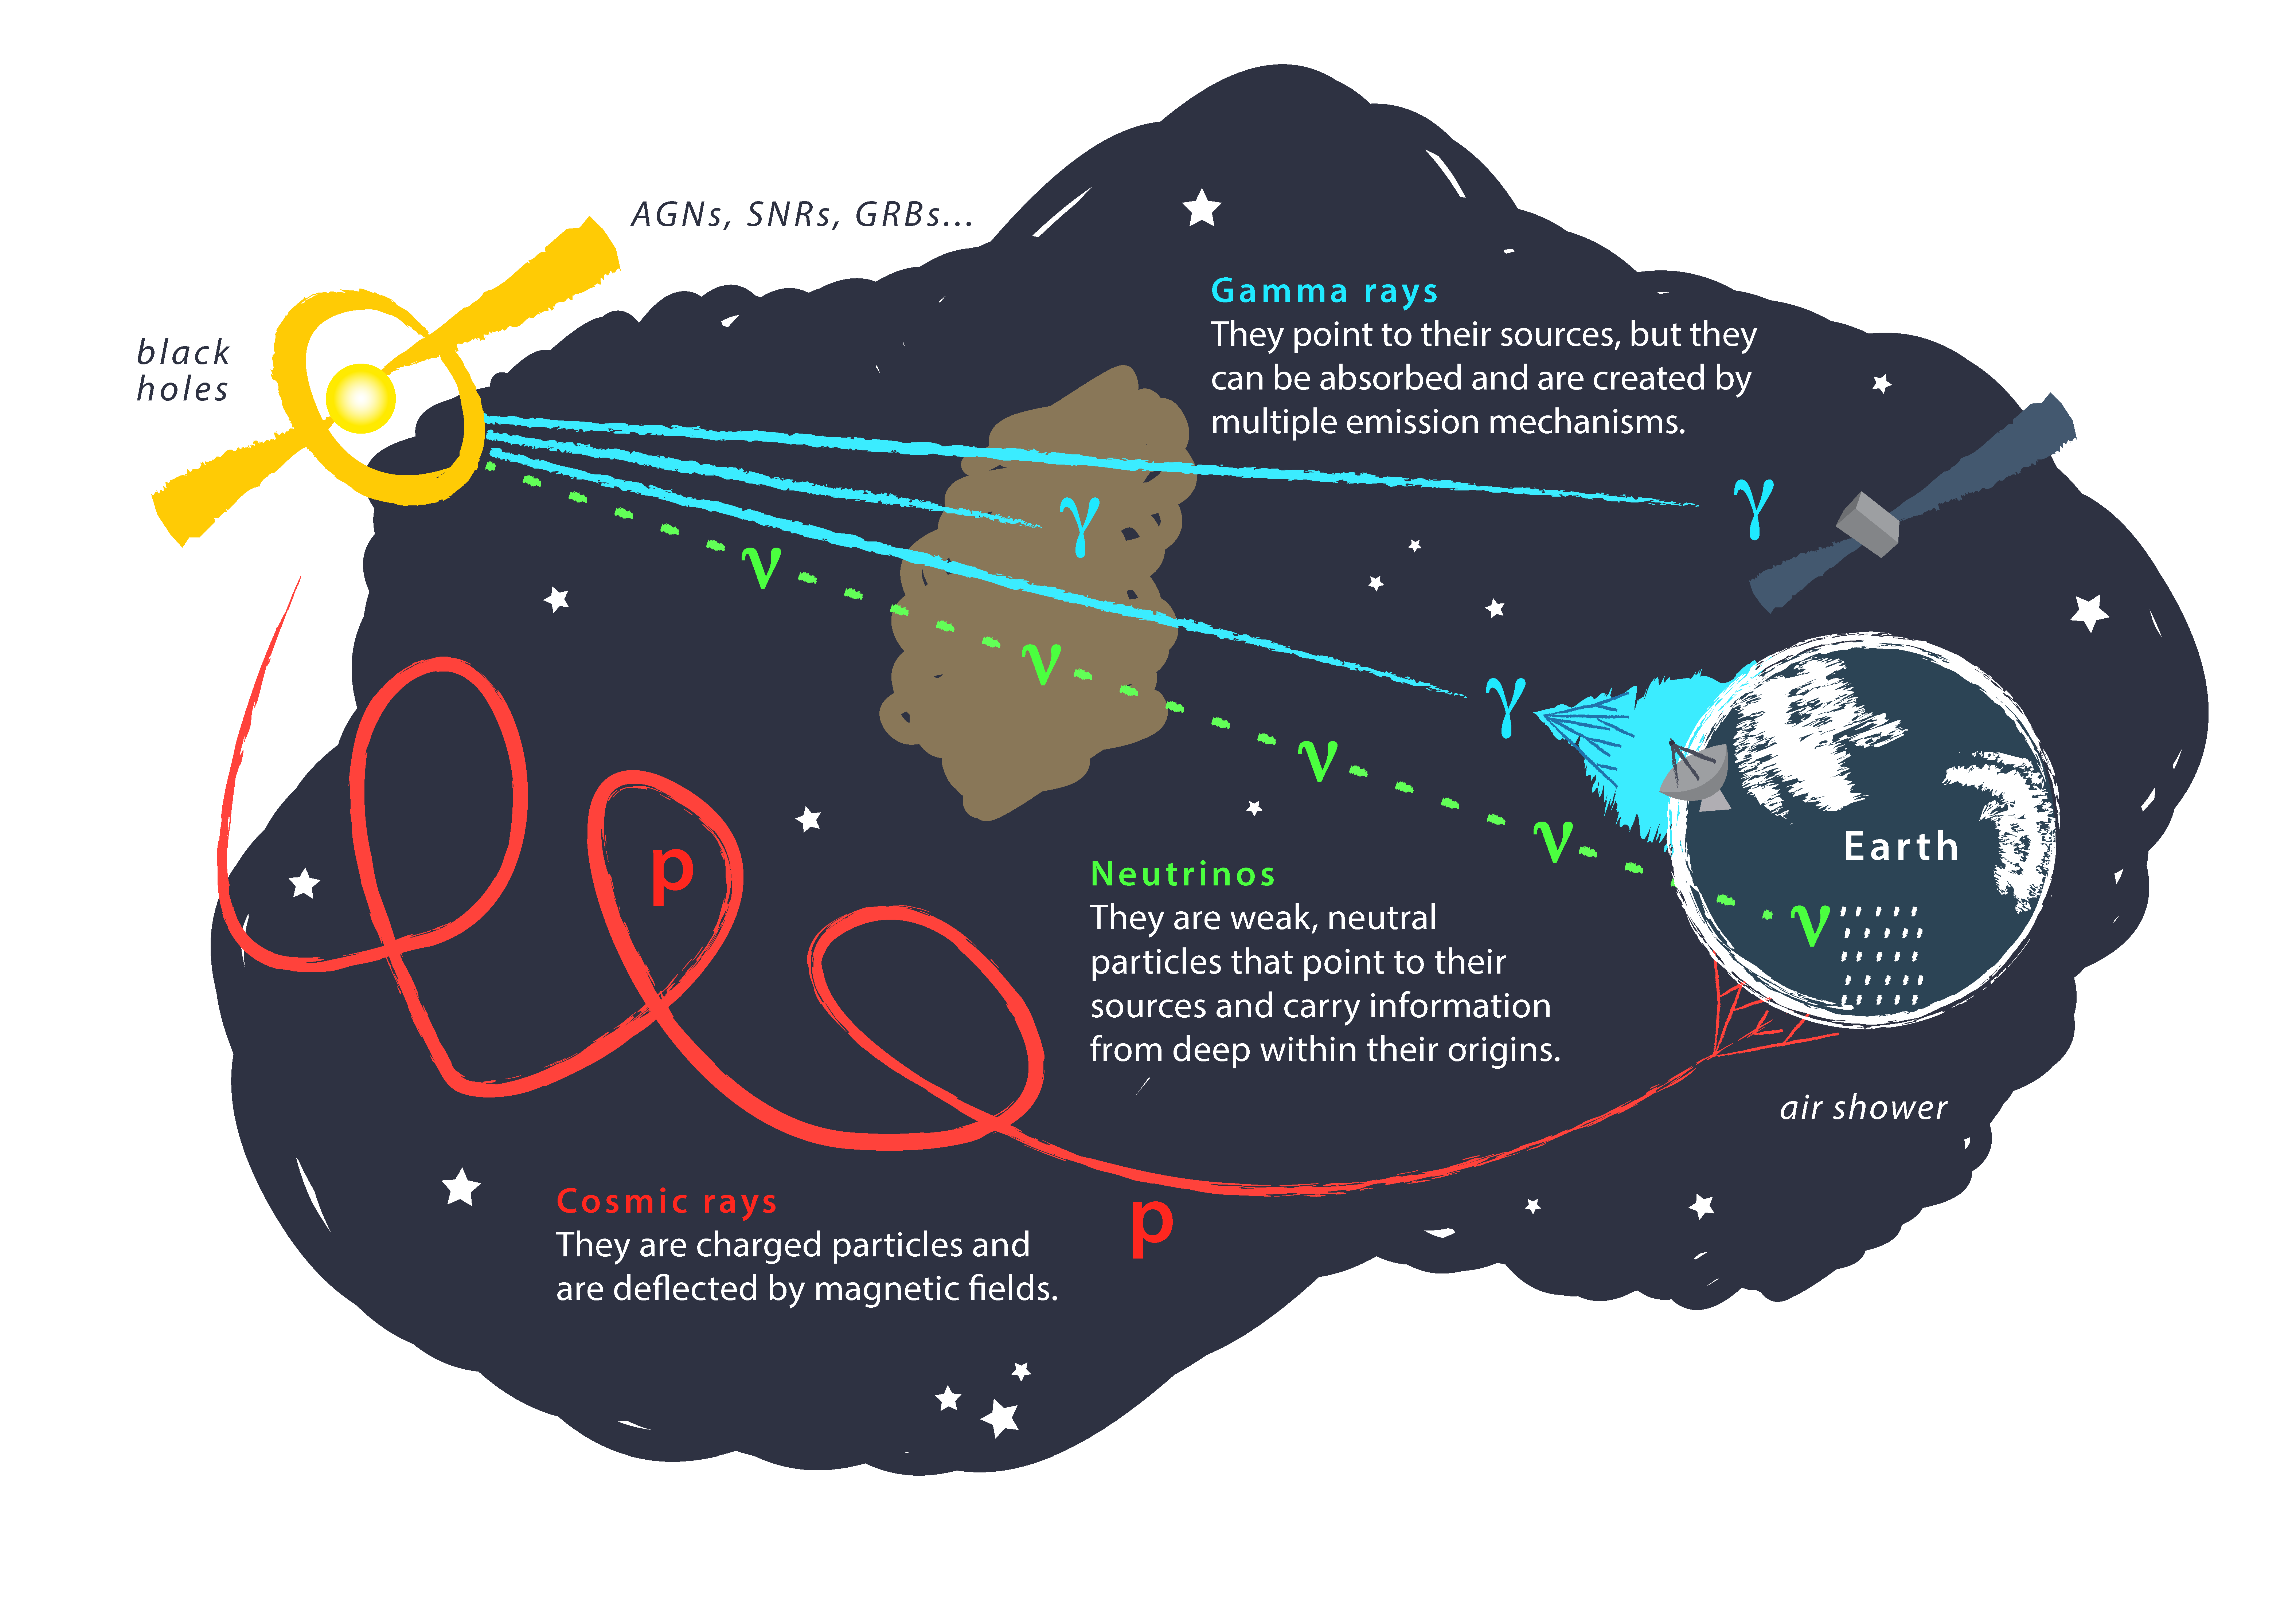
\includegraphics[width=0.9\textwidth]{images/cosmic_messengers.png}
    \caption{Only uncharged particles carry information about their origin when they arrive on earth.
        Neutrinos are hard to detect as they only interact via the weak force.
        Photons on the other hand can be absorbed in gas clouds, but are detectable using satellite- and ground-based observeratories.
    }
    \label{fig:mma}
\end{figure}

Photons and neutrions are of special interest as they are not influenced by cosmic electromagentic fields and therefore it is possible to reconstructed their origin 
position and study their sources.
As high energy gamma radiation cannot be produced thermally, more complex processes involving charged particles (Cosmic Rays) have to be considered 
(Further information in \cite{s_funk}).

The most important source class within our own galaxy are supernova remnants like the Crab Nebula \cite{nuimeprn12618}. 
Because of its constantly high gamma ray flux the Crab Nebula is often used as a "standart candle" in Gamma Ray Astronomy, observations of which are also 
analysed as part of this work.
Extragalactic sources for gamma rays are mostly supermassive black holes at the center of very bright galaxies, so called active galactic nuclei (AGN).
These black holes accrete matter from its surroundings resulting in the formation of disks around the black holes and sometimes relativistic jets are emitted 
perpendicular to the disk.
AGNs are classified depending on if a jet is emitted, how bright they are and at which angle they are observed as shown in \autoref{fig:agn}.
One of closest to earth examples of a blazar is Markarian 421 located at a redshift of $z = \num{0.03}$ \cite{Albert_2007} and observations of it are analysed in 
\autoref{ch:results}.
\begin{figure}
    \centering
    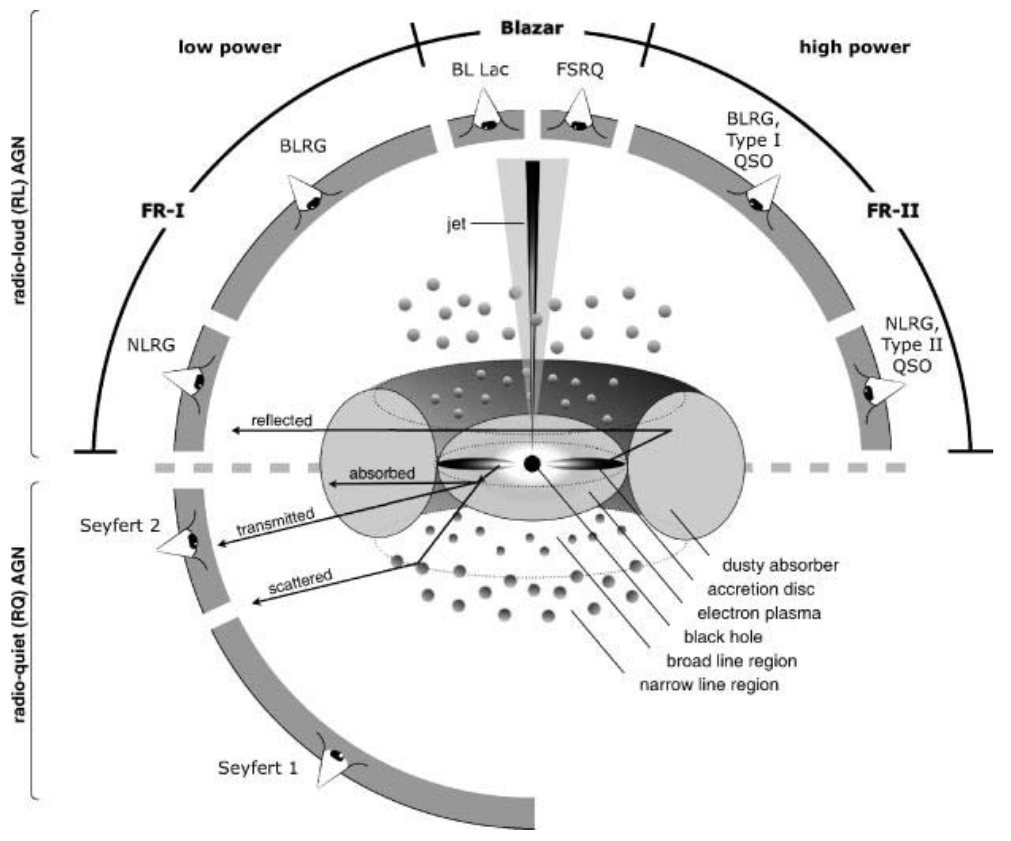
\includegraphics[width=0.8\textwidth]{images/agn.png}
    \caption{AGNs consist of a supermassive black hole in the center surrounded by an accretion disc which is again surrounded by a gas torus.
        The calssification of AGNs is based on three main characteristics, the existence of a jet, their brightness and the angle under which they can be observed \cite{doi:10.1002/9783527666829.ch4}.
    }
    \label{fig:agn}
\end{figure}


As earth's atmosphere is not transparent for high energy gamma rays, direct observations of gamma rays can only be done by satellite based observeratories 
like the Large Area Telescope on the \textit{Fermi} Gamma-Ray Space Telescope (\textit{Fermi}-LAT).
On the ground indirect observations are possible by using Imaging Air Cherenkov Telescopes (IACTs) which will be explained further in \autoref{ch:cta}.

\chapter{Imaging Air Cherenkov Telescopes and the Cherenkov Telescope Array}
\label{ch:cta}

\section{Imaging Air Cherenkov Telescopes}
For IACTs the atmosphere itself acts as the detector medium. 
If a high energy primary particle interacts with the atmosphere it starts a cascade of secondary paricles called air showers.
The charged secondary particles travel faster than the speed of light in air resulting in the emission of Cherenkov Light.
This light is emitted along the moving direction of the charged particle.
The Cherenkov Light is then collected by mirrors and projected onto a camera system which is able to record single photons with a time resolution of a few nanoseconds.

As both charged primary paricles and photons start air showers a dominant background of hadronic air showers is recorded by IACTs.
In hadronic air showers many different interactions are possible due to the strong force.
These varied interactions lead to the more complex shower pattern of hadronic air showers resulting in the possibility to distinguish them from purely electromagnetic
air showers caused by photons or electrons.
Electromagnetic air showers only consist of two processes. 
High energy photons produce electron-positron pairs and the total energy of those two paricles equals the photon energy. 
High energy electrons/positrons then generate photons again through bremsstahlung. 
These two processes continue until the photon energy falls under energy threshold for pair production of $\SI{1022}{\kilo\electronvolt}$.


\section{CTA and the LST-1 prototype}
The Cherenkov Telescope Array (CTA) aims to be the next generation IACT experiment by providing a sensitivity at least an order of magnitude better than current experiments.
It will be comprised of two sites, one in the northern and one in the southern hemisphere which will consist of differently sized telescopes. 
The smallest one will be the Small-Sized Telescope (SST) sensitive for the highest energies above $\SI{5}{\tera\electronvolt}$ up until $\SI{300}{\tera\electronvolt}$.
The Medium-Sized Telescope (MST) is most sensitive for energies between $\SI{150}{\giga\electronvolt}$ and $\SI{5}{\tera\electronvolt}$ and the 
Large-Sized Telescope (LST) will cover the lowest energies from $\SI{20}{\giga\electronvolt}$ up until $\SI{150}{\giga\electronvolt}$.
A size comparsion of the telescopes can be seen in \autoref{fig:telescopes}.
\begin{figure}
    \centering
    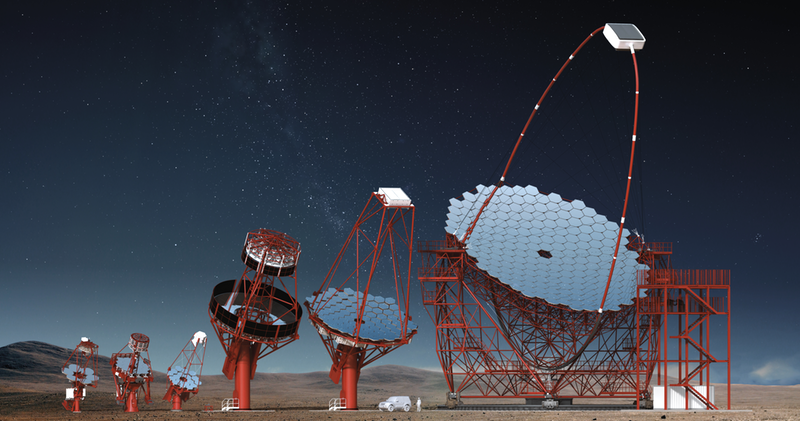
\includegraphics[width=0.8\textwidth]{images/CTA_telescopes.png}
    \caption{A depiction of the different telescopes that will be used to build CTA. 
        Three prototypes are currently being tested for the SST, two for the MST and one for the LST \cite{cta-website}.
    }
    \label{fig:telescopes}
\end{figure}

The southern site will be located in the Atacama desert in Chile and will consist of \num{4} LSTs, \num{25} MSTs and \num{70} SSTs.
The northern site will be build as part of the Observatorio del Roque de los Muchachos (ORM) on LaPalma and will include \num{4} LSTs and \num{15} MSTs.
More information about the CTA and its scientific capabilities can be found in \cite{science_with_cta}.

***More info about the sites/SST, MST ?***

The ORM is also the location of the first prototype for the LSTs inaugurated on the 10 October 2018, the LST-1 which is the subject of this work \cite{lst_inauguration}.
The LST-1 has a parabolic mirror with a diameter of $\SI{23}{\meter}$ which helps to collect the Cherenkov light of the dimmest low-energy air showers.
The light is recorded by a $\num{1855}$-pixel camera based on photomultiplier tubes with a field of view of about $\SI{4.3}{\degree}$ \cite{cta-website}.


\chapter{Preprocessing of the data}
\label{ch:prepro}

Before the analysis steps done in this work can be performed, the raw data taken by the LST-1 has to be processed up until what is called Data Level 1 (DL1).
For this work such preprocessing was done using \texttt{lstchain}, a low-level data processing pipeline for the LST telescopes. 
\texttt{lstchain} is open-source project which is still in development on github \cite{lstchain} and is based on \texttt{ctapipe}. 
\texttt{ctapipe} will be the main low-level data processing pipeline for CTA and is itself in development as an open-source project.
This work uses the versions \texttt{v0.5.1} and \texttt{v0.5.2} of \texttt{lstchain} which are both based on version \texttt{v0.7.0} of \texttt{ctapipe} \cite{ctapipe}. 

In the first step the waveforms recorded by each pixel of the camera are cleaned to reduce the influence of electronic noise in the signal.
After that the waveforms are integrated to obtain the total photon charge and a mean arrival time for the photons is defined for each pixel 
as the point in time at which half of all the photons within the pixel have arrived.
This results in two 2-dimensional images for each event recorded by the camera, as can be seen in \autoref{fig:eas_images}.
\begin{figure}
    \centering
    \begin{subfigure}{0.49\textwidth}
        \centering
        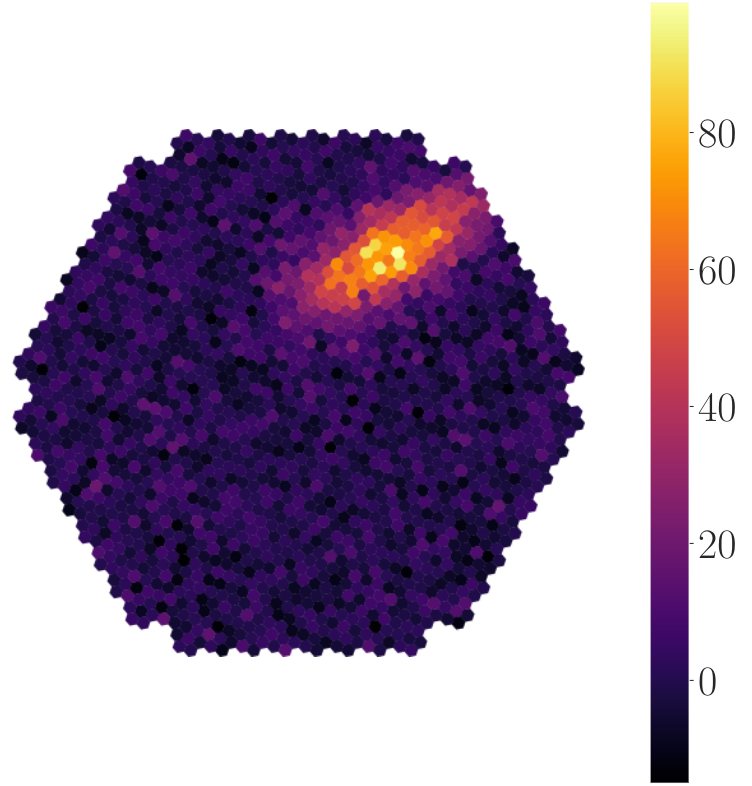
\includegraphics[width=0.8\textwidth]{images/eas_image1.png}
        \caption{Number of photons per pixel.}
        \label{fig:eas_image1}
    \end{subfigure}
    \hfill
    \begin{subfigure}{0.49\textwidth}
        \centering
        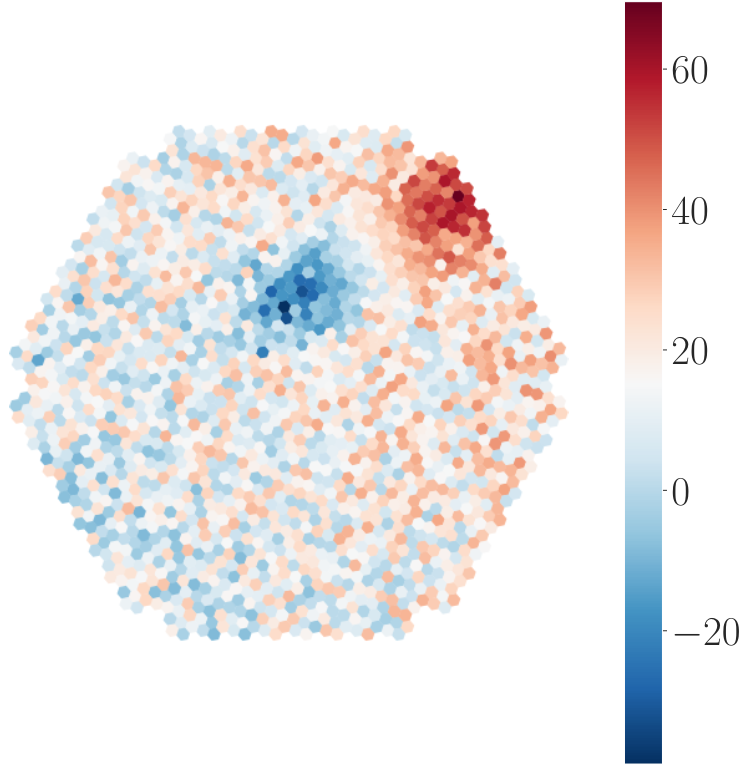
\includegraphics[width=0.8\textwidth]{images/eas_image2.png}
        \caption{Arrival time per pixel relative to the mean arrival time for the whole image.}
        \label{fig:eas_image2}
    \end{subfigure}
    \caption{The integrated photon count in \subref{fig:eas_image1} showes the air shower clearly but a lot of noise is visible in the non-shower pixels.
        The arrival times in \subref{fig:eas_image2} show a clear correlation for the pixels that recorded the air shower \cite{lukas}.
    }
    \label{fig:eas_images}
\end{figure}

In the next step these images are cleaned by discarding pixels that did not record the air shower. 
This is done in multiple steps using two thresholds for the photon charge of each pixel and one for the number of neighboring pixels.
First all pixels above the higher photon charge threshold with enough neighboring pixels above the lower photon charge threshold get selected as part of the shower.
After that all pixels above the lower photon charge threshold with enough neighboring pixels above the higher photon charge threshold get selected as well \cite{lukas}.
For rather soft thresholds the results of this cleaning can be seen in \autoref{fig:eas_images_cleaned}.
\begin{figure}
    \centering
    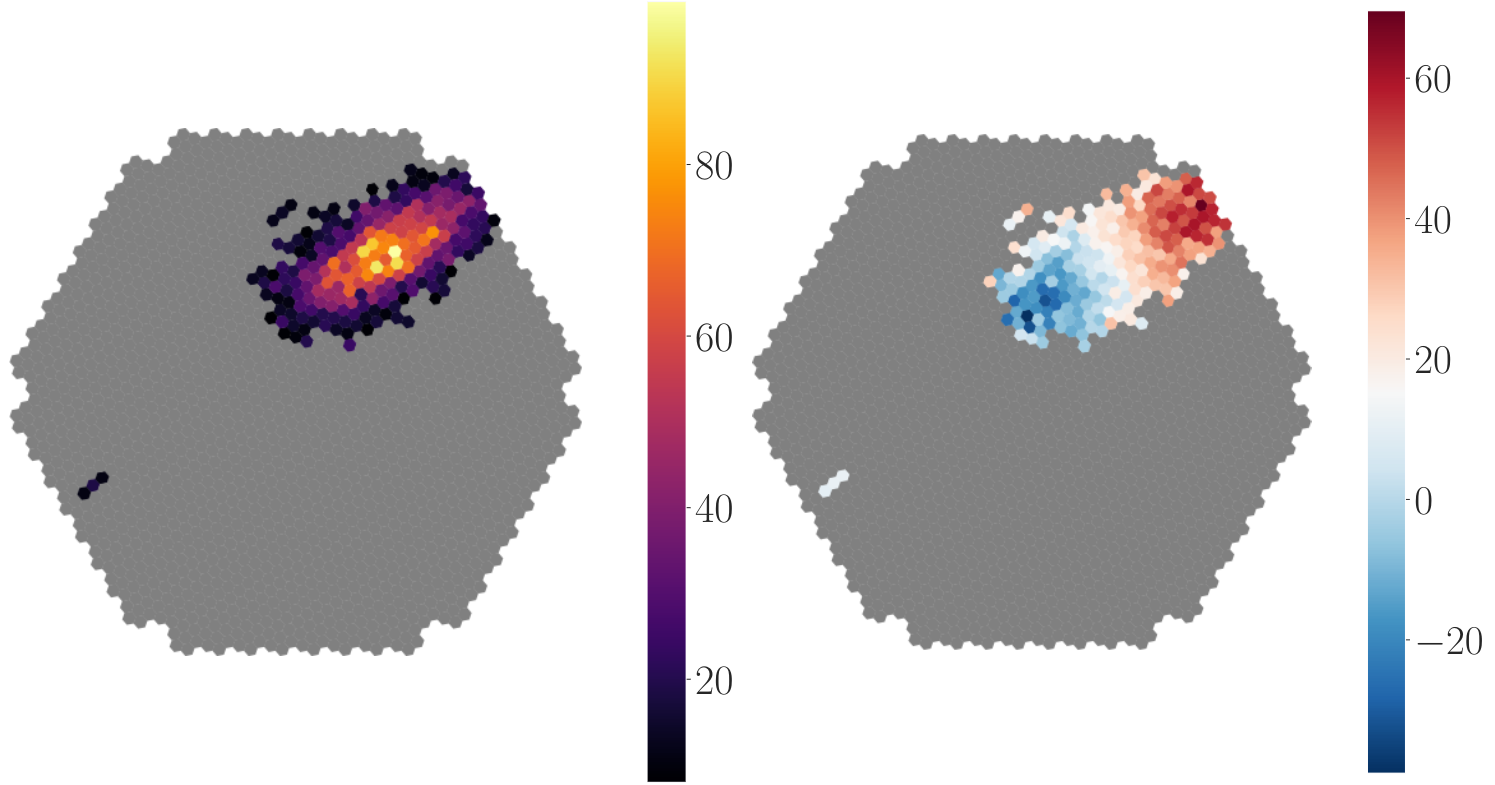
\includegraphics[width=0.8\textwidth]{images/eas_images_cleaned.png}
    \caption{The pixels discarded during the image cleaning are marked as grey. The soft thresholds chosen for this example result in two smaller pixel-islands remaining \cite{lukas}.}
    \label{fig:eas_images_cleaned}
\end{figure}

Based on these cleaned images, a multitude of image parameters can be calculated.
The most important ones are the total number of photons in the shower, \texttt{intensity}, and the so called hillas parameters which are illustrated in \autoref{fig:image_parameters}.
the hillas parameters are based on a principal component analysis (PCA) of the photon charge distribution and describe the extension and orientation of the shower.
The parameters \texttt{length} and \texttt{width} correspond with the standard deviations along the principal components of the distribution and are therefore a 
description of the shower extension. 
The orientation on the other hand is described by the angle of the main shower axis relative to the $x$-axis of the image.
The performance of the algorithms used in this work in regards to reconstructing this angle can be seen in \autoref{fig:delta_comparison}.
\begin{figure}
    \centering
    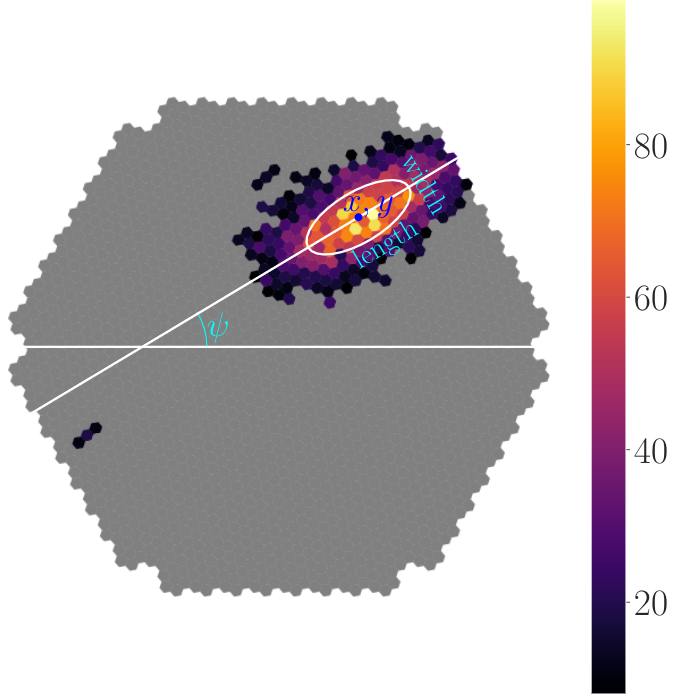
\includegraphics[width=0.5\textwidth]{images/image_parameters.png}
    \caption{The PCA-based hillas-parameters calculated for the cleaned image of the integrated photon count.
        $\Psi$ describes the angle of the main shower axis relative to the x-axis of the image and $x$ and $y$ are the coordinates of the center of gravity of the shower. 
        \texttt{length} and \texttt{width} can be depicted as the semi-major and semi-minor axis of an ellipse \cite{lukas}.
    }
    \label{fig:image_parameters}
\end{figure}

Higher moments of the distribution like \texttt{skewness} and \texttt{kurtosis} are also calculated. 
The center of gravity of the shower image is calculated by weighting the coordinates of each pixel with the photon charge of this pixel.
Additional image featueres include multiple \texttt{leakage} parameters that describe how much of the light was recorded at the edge of the camera and are
therefore an indication of how much light from the shower might have missed the camera.

The image of the arrival times allows for timing parameters to be calculated by fitting a linear function along the main shower axis. 
This yields the parameters \texttt{time\_gradient} and \texttt{intercept} which help to determine the direction of the shower, together with \texttt{skewness}.
\chapter{Reconstruction of physical properties using machine learning}
\label{ch:ml}
Using the image parameters for each event, the particle type, origin and energy of the primary particle can be reconstructed.
In this work, supervised machine learning is used for the reconstruction.
The algorithms are trained on a set of Monte Carlo simulations which are preprocessed using two different versions of \texttt{lstchain} 
and the results are compared in \autoref{ch:results}.
The set includes a simulation of the detection of diffuse gamma rays, diffuse protons and a simulation of gamma rays emitted by a point-like source.
The simulations were done using the programs \texttt{CORSIKA} and \texttt{sim\_telarray} \cite{simulations}.

In supervised machine learning a generic estimator $f$ is trained on a dataset for which all information is known.
Training means that the parameters of $f$ get fitted in order to minimize a loss-function for certain target features.
This trained estimator, or model, can then be used to estimate the target features of datasets where this information is missing.

Two common types of problems that can be solved this way are binary classification and regression. 
For binary classification problems the estimator $f$ has to guess which of two classes any given element is a part of. 
This is used for background separation and during the origin reconstruction.
To solve a regression problem a countinuous quantity has to be estimated which is used for energy estimation and again during origin reconstruction.

It is important to validate the trained models before using them to estimate unknown features.
This is done by applying them to a different dataset than the dataset the model was trained on, but for which all information is known as well.
This allows for a comparison between the estimated values and the true values for the target features which is necessary to prevent overfitting.
Overfitting means that the model learned the training dataset \enquote{by heart} and did not recognize the underlying structure and is therefore not able
to estimate features for other datasets.

In this work, a $\num{5}$-fold cross validation is used which means that the training dataset is split into $\num{5}$ parts and training happens 
with $\num{4}$ of those parts while the remaining part is used for validation. 
The training is done on all possible combinations of the $\num{4}$ parts resulting in $\num{5}$ training sets.


\section{Decision Trees and Random Forests}
The basis for the random forest algorithm is the decision tree algorithm \cite{breiman1984classification} or more specifically binary trees.
A binary tree splits a dataset into two subsets at each step, called node.
For each split a threshold $t_j$ for a certain feature $j$ is chosen that minimizes the given loss-function.
This is repeated recursively until a stopping criterion is met like e.g. a maximum number of nodes (\enquote{depth} of the tree). 
The final subsets are called leafs and for binary classification partition between the two classes within each leaf is returned as a prediction threshold
$t_p \in [0,\, 1]$.
For a regression task the average value of the regression target feature within each leaf is returned.

One common loss-function for binary classification is the cross-entropy
\begin{align}
    \text{Cross-entropy} = - p\, \log(p) - (1 - p) \log(1-p)
\end{align}
with $p$ being the proportion of one of the two classes.
For the regression problem the mean squared error is often used as loss function which is evaluated for all $j$ features in every node \cite{hastie2009elements}.
\begin{align}
    \text{mse} = \sum_{X_{i,j} \in\, R_1} (y_i - c_1)^2\, + \sum_{X_{i,j} \in\, R_2} (y_i - c_2)^2,
\end{align}

As decision trees have some weaknesses like an inherent instability, Leo Breimann introduced the random forest algorithm \cite{breiman2001random}. 
This algorithm trains multiple decision trees on slightly different datasets which are created from the initial training dataset by sampling with replacement.
This process is called bagging \cite{breiman1996bagging}.
To add even more randomness to the training only a random subsample off all given features is considered in each node. 
The results from these trees are then averaged.


\section{Quality Metrics}
\label{sec:quality_metrics}
To quantify the performance of a model there are a number of quality metrics for binary classification which are all based on the confusion matrix.
\begin{align}
    \begin{pmatrix}
        tp & fp \\
        fn & tn
    \end{pmatrix}
\end{align}
$tp$ means \enquote{true postives} and $tn$ means \enquote{true negatives}. 
These two values describe the proportion of correctly classified members of the two classes (\enquote{postive} and \enquote{negative}).
$fp$ (\enquote{false positives}) and $fn$ (\enquote{false negatives}) on the other and describe the amount of falsely classified members of the two classes respectively.
In this work, the following metrics are used based on this connotation.
\begin{itemize}
    \item \textbf{Precision} represents the percentage of correctly classified members of the reconstructed \enquote{positive} class.
        \begin{align}
            \text{precision} = \frac{tp}{tp\, +\, fp}
        \end{align}
    \item \textbf{Recall} describes the ability of the classifier to identify members of the \enquote{positive} class as such.
        \begin{align}
            \text{recall} = \frac{tp}{tp\, +\, fn}
        \end{align}
    \item \textbf{Accuracy} measures the overall percentage of correctly reconstructed samples.
        \begin{align}
            \text{accuracy} = \frac{tp\, +\, tn}{tp\, +\, tn\, +\, fp\, +\, fn}
        \end{align}
    \item \textbf{$\text{F}_\beta$-Score} is the weighted harmonic mean of precision and recall where the weight $\beta$ can be chosen to emphasize recall or precision.
        \begin{align}
            f_\beta = (1 + \beta^2) \frac{\text{precision}\, \cdot\, \text{recall}}{\beta^2\, \text{precision}\, +\, \text{recall}}
        \end{align}
\end{itemize}
It is also of interest to examine the classifier performance independent of the prediction threshold $t_p$ 
(which requires a metric thats independent of the confusion matrix).
A common metric for this is the area under the Receiver Operating Characteristic (ROC) curve.
In the ROC curve the $tp$ rate is plotted against the $fp$ rate for every possible threshold $t_p$.

For regression models the coefficient of determination or $r^2$-score is often used as quality metric.
\begin{align}
    r^2 = 1 - \frac{\sum_{i = 0}^N (y_i - \hat{y}_i)^2}{\sum_{i = 0}^N (y_i - \bar{y})^2}
\end{align}
$\hat{y}_i$ is the estimated value for the true value $y_i$ and $\bar{y}$ is the arithmetic mean of all $y_i$.


\section{The aict-tools}
For the training and appliction of such models in the context of data analysis for IACTs the command line tools from the \texttt{aict-tools} package can be used \cite{aict-tools}. 
For the implementation of the machine learning algorithms the \texttt{aict-tools} use the \texttt{scikit-learn} module \cite{scikit-learn}.
The configuration of models is done using a single \text{yaml}-file and the configuration used in this work can be found in \autoref{sec:config}.

Initially the \texttt{aict-tools} were developed for the FACT-experiment which uses a different coordinate system and data-structure than CTA.
Therefore at the start of this work some conversion of the LST-1 data had to be done before the \texttt{aict-tools} could be applied.
Due to the continued developed of the \texttt{aict-tools} different coordinate systems are now supported and the necessary conversions became largely obsolete.
By the time of writing merely the data-structure of the LST-1 data has to be adjusted before the \texttt{aict-tools} can be applied.

Another utility provided by the \texttt{aict-tools} is the generation of additional custom image features based on existing ones.
This is utilized in this work and the features that are generated can be seen in \autoref{sec:config}. 
The calculation of the quality metrics presented in \autoref{sec:quality_metrics} is also done using their appropriate implementation in the \texttt{aict-tools}.


\section{The DISP method}
The estimation of the origin within the detector plane normally results in a two dimensional regression task ($x$ and $y$).
The \texttt{aict-tools} use the disp methode instead which simplifies this task into a one dimensional regression task and a binary classification.

This is done by assuming the main shower axis as correctly reconstructed so that the origin of the primary particle lies somewhere along this line.
Based on this, the regression task aims to determine the absolute distance of the origin from the center of gravity of the shower image called \texttt{|disp|}.
As the regression results in two possible origin positions along the main shower axis, the objective of the binary classification is to decide which
of those two is the correct origin position.
This is called \texttt{sign} of disp.

\chapter{Results}
\label{ch:results}
Preprocessing of the first set of simulations (without the scaling of the optical efficiency) as well as the observational data for the Crab Nebula and 
Markarian 421 was done using \texttt{v0.5.1} of \texttt{lstchain}.
The second set of simulations (with the scaling of the optical efficiency) was processed using \texttt{v0.5.2}.
Hereafter the different sets of simulations will be referred to by the respective versions of \texttt{lstchain} they were processed with.

Before training the machine learning models a pre-selection of the events for the simulations as well as the observational data is done to remove 
hard to reconstruct and not properly simulated events. 
This pre-selection can also be done using the \texttt{aict-tools}.
For this work two different sets of criteria are used and the different results are compared in \autoref{ch:results}.
\begin{align*}
    &\underline{\textbf{criteria-set 1:}} & &\underline{\textbf{criteria-set 2:}} \\
    &\texttt{intensity > 300} & &\texttt{intensity > 150} \\
    &\texttt{leakage1\_intensity < 0.2} & &\texttt{leakage1\_intensity < 0.2} \\
    &\texttt{leakage2\_intensity < 0.2} & &\texttt{leakage2\_intensity < 0.2}
\end{align*}

\section{Model performance}


\section{Observations of the Crab Nebula}


\section{Observations of Markarian 421}

\chapter{Outlook}

\appendix
% Hier beginnt der Anhang, nummeriert in lateinischen Buchstaben
\chapter{Appendix}

\section{Reconstruction of main shower axis angle}
\begin{figure}
    \centering
    \begin{subfigure}{0.49\textwidth}
        \centering
        \includegraphics[width=\linewidth]{build/plots_disp/plot_7.pdf}
        \caption{\texttt{lstchain v0.5.2} and \texttt{intensity > 150}.}
        \label{fig:newMC_150}
    \end{subfigure}
    \hfill
    \begin{subfigure}{0.49\textwidth}
        \centering
        \includegraphics[width=\linewidth]{HDD/build_scaling_300/plots_disp/plot_7.pdf}
        \caption{\texttt{lstchain v0.5.2} and \texttt{intensity > 300}.}
        \label{fig:newMC_300}
    \end{subfigure}
    \newline\vfill
    \begin{subfigure}{0.49\textwidth}
        \centering
        \includegraphics[width=\linewidth]{HDD/build_noscaling_300/plots_disp/plot_7.pdf}
        \caption{\texttt{lstchain v0.5.1} and \texttt{intensity > 300}.}
        \label{fig:newMC_300}
    \end{subfigure}
    \caption{A histogram of the difference between the reconstructed main shower axis angle $\delta$ and the true simulated main shower axis angle $\delta_\text{true}$.
        In all three cases the reconstruction works well, as a difference of $\num{0}$ and $\pm \pi$ means that the angle was reconstructed correctly.
    }
    \label{fig:delta_comparison}
\end{figure}



\section{Configuration of the aict-tools}
\label{sec:config}
\begin{verbatim}
seed: 0
true_energy_column: mc_energy
energy_unit: TeV

multiple_telescopes: False

n_cross_validations : 5

separator:
  classifier : |
    ensemble.RandomForestClassifier(
        n_estimators=100,
        max_features='sqrt',
        n_jobs=-1,
        max_depth=15,
        criterion='entropy',
    )

  # randomly sample the data if you dont want to use the whole set
  n_background: 50000
  n_signal: 50000

  # Define the name of the output column for the positive class.
  output_name: gammaness

  features:
    - intensity
    - log_intensity
    - intercept
    - time_gradient
    - length
    - width
    - skewness
    - kurtosis
    - n_islands
    - n_pixels
    - leakage1_intensity
    - leakage1_pixel
    - leakage2_intensity
    - leakage2_pixel
    - concentration_cog
    - concentration_core
    - concentration_pixel

  # Generate some features using pd.DataFrame.eval
  feature_generation:
    needed_columns:
      - width
      - length
      - intensity
    features:
      area: width * length * @pi
      intensity_area: intensity / (width * length * @pi)
      area_intensity_cut_var: (width * length * @pi) / log(intensity)**2

disp:
  disp_regressor : |
    ensemble.RandomForestRegressor(
        n_estimators=100,
        max_features='sqrt',
        n_jobs=-1,
        max_depth=20,
    )

  sign_classifier: |
    ensemble.RandomForestClassifier(
        n_estimators=100,
        max_features='sqrt',
        n_jobs=-1,
        max_depth=20,
    )

  coordinate_transformation: CTA

  source_az_column: mc_az
  source_az_unit: rad
  source_alt_column: mc_alt 
  source_alt_unit: rad
  pointing_az_column: az_tel
  pointing_az_unit: rad
  pointing_alt_column: alt_tel
  pointing_alt_unit: rad

  cog_x_column: x  
  cog_y_column: y  
  delta_column: psi
  delta_unit: rad
  focal_length_column: focal_length
  focal_length_unit: m

  # randomly sample the data if you dont want to use the whole set
  n_signal : 50000

  features:
    - intensity
    - log_intensity
    - width
    - length
    - n_pixels
    - leakage1_intensity
    - leakage1_pixel
    - leakage2_intensity
    - leakage2_pixel
    - r
    - kurtosis
    - skewness
    - concentration_cog
    - concentration_core
    - time_gradient
    - intercept

  feature_generation:
    needed_columns:
      - width
      - length
      - log_intensity
    features:
      elongation: width / length
      area: width * length * @pi
      log_intensity_area: log_intensity / (width * length * @pi)

energy:
  regressor : |
    ensemble.RandomForestRegressor(
      n_estimators=100,
      max_features='sqrt',
      n_jobs=-1,
      max_depth=12,
    )

  # randomly sample the data if you dont want to use the whole set
  n_signal: 50000

  # define the name of the regression target
  target_column: mc_energy
  log_target: true

  # Define the name of the variable you want estimate by regression.
  output_name: gamma_energy_prediction

  features:
    - intensity
    - log_intensity
    - length
    - width
    - n_islands
    - n_pixels
    - skewness
    - leakage1_intensity
    - leakage1_pixel
    - leakage2_intensity
    - leakage2_pixel
    - concentration_cog
    - concentration_core
    - concentration_pixel

  # Generate some features using pd.DataFrame.eval
  feature_generation:
    needed_columns:
      - width
      - length
      - intensity
    features:
      area: width * length * @pi
      intensity_area: intensity / (width * length * @pi)
\end{verbatim}

\backmatter
\printbibliography

\cleardoublepage
\thispagestyle{empty}
\section*{Eidesstattliche Versicherung}
Ich versichere hiermit an Eides statt, dass ich die vorliegende Abschlussarbeit mit dem Titel \enquote{\thetitle} selbstständig und ohne unzulässige fremde Hilfe erbracht habe.
Ich habe keine anderen als die angegebenen Quellen und Hilfsmittel benutzt, sowie wörtliche und sinngemäße Zitate kenntlich gemacht. 
Die Arbeit hat in gleicher oder ähnlicher Form noch keiner Prüfungsbehörde vorgelegen.

\vspace*{1cm}\noindent
\begin{center}
  \begin{tabular}{@{}p{0.4\textwidth}@{\hspace{0.15\textwidth}}p{0.4\textwidth}@{}}
  \rule{\linewidth}{0.25pt}& \rule{\linewidth}{0.25pt}\\
  Ort, Datum & Unterschrift
  \end{tabular}
\end{center}

\subsection*{Belehrung}
Wer vorsätzlich gegen eine die Täuschung über Prüfungsleistungen betreffende Regelung einer Hochschulprüfungsordnung verstößt, handelt ordnungswidrig.
Die Ordnungswidrigkeit kann mit einer Geldbuße von bis zu \SI[round-mode=places, round-precision=2]{50000}{€} geahndet werden. 
Zuständige Verwaltungsbehörde für die Verfolgung und Ahndung von Ordnungswidrigkeiten ist der Kanzler/die Kanzlerin der Technischen Universität Dortmund. 
Im Falle eines mehrfachen oder sonstigen schwerwiegenden Täuschungsversuches kann der Prüfling zudem exmatrikuliert werden \mbox{(\S\,63 Abs. 5 Hochschulgesetz --HG--).}

Die Abgabe einer falschen Versicherung an Eides statt wird mit Freiheitsstrafe bis zu 3 Jahren oder mit Geldstrafe bestraft.

Die Technische Universität Dortmund wird ggf.\ elektronische Vergleichswerkzeuge (wie z.\,B.\ die Software \enquote{turnitin}) zur Überprüfung von Ordnungswidrigkeiten in Prüfungsverfahren nutzen. \\[\baselineskip]

\noindent Die oben stehende Belehrung habe ich zur Kenntnis genommen.\\[1cm]
\begin{center}
\begin{tabular}{@{}p{0.4\textwidth}@{\hspace{0.15\textwidth}}p{0.4\textwidth}@{}}
\rule{\linewidth}{0.25pt}& \rule{\linewidth}{0.25pt}\\
Ort, Datum & Unterschrift
\end{tabular}
\end{center}

\end{document}
